% add your introduction section here ...
``\textit{This includes examples of quotes, the inclusion and reference to a Figure, a (chapter-specific) citation and a summary box.}''\\
\hspace*{.83\textwidth}{\citepim{Darwin1859_i}} %note the section-specific citation commands (indication section and within text (i/a/b/c/z), and self reference from the chapter title (p/m))

\begin{multicols}{2}
\begin{figure*}[!hb] % figure will be placed after the next paragraph finishes
\centering
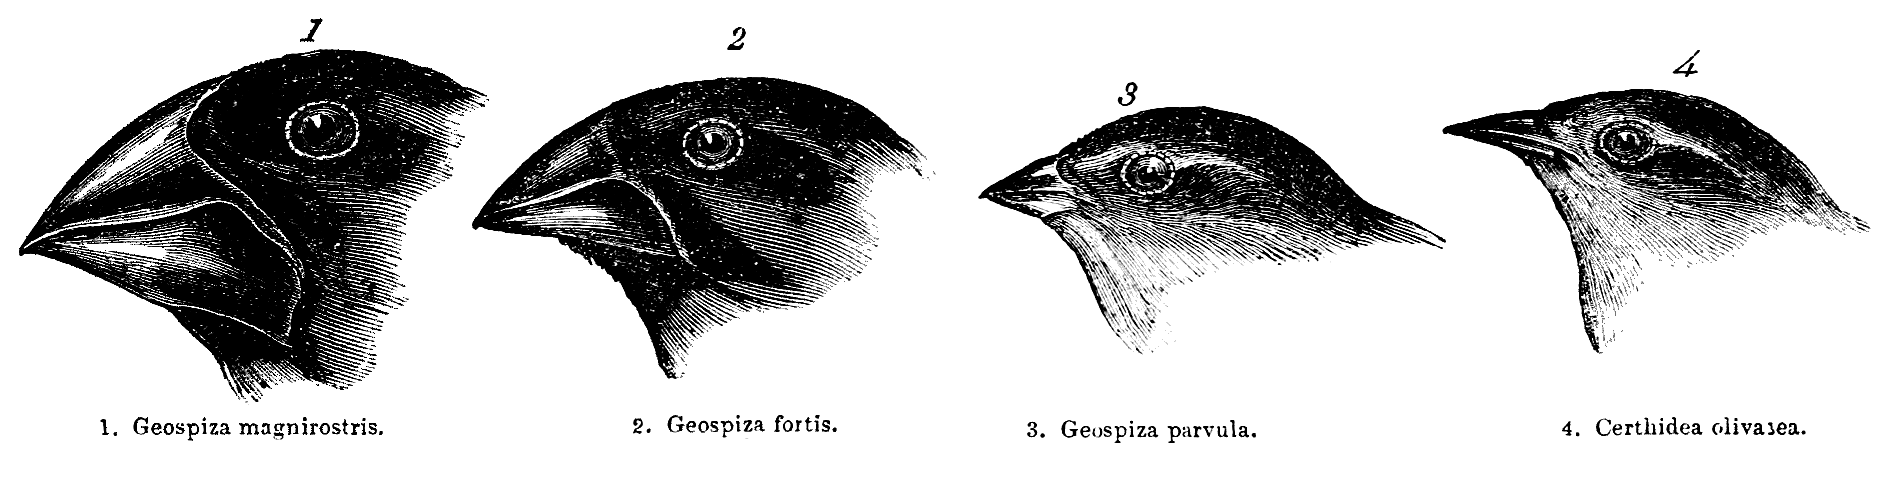
\includegraphics[width = \fwidth]{figures/ci/finches.png}
\caption[Darwins Finches]{\label{fig:cif1}\textbf{Darwins Finches.} These are such famous birds.
}
\end{figure*}

\section{First Section}

\textbf{Inline Quotes:} By the way, we can also quote \textit{in line} using the environment \texttt{$\backslash$displayquote}:

\begin{displayquote}
\textit{
I look at the term species, as one arbitrarily given for the sake of convenience to a set of individuals closely resembling each other [...].}
\hfill{\citepim{Darwin1859_i}}
\end{displayquote}

\textbf{Adding Figures:}
Figures are added to the text using the \texttt{figure*} environment in combination with the \texttt{$\backslash$includegraphics} command (s. example in source code).
You can also use the \texttt{$\backslash$label} command to add a tag to the figure which you can use to refernce the figure in your text.
Note that figures will show up somewhere \textit{after} the paragraph that follows the \textsw{figure*} environment. If you need to force the appearance on a specific page you can use the command \texttt{$\backslash$FloatBarrier}.

Here is some demonstration how to reference a Figure (using the label from the figure command) --- just look at these birds (\figref{fig:cif1}).
The reference is done using the command \texttt{$\backslash$figref\{\}}.

\textbf{Landscape Figures:} For figures in \textit{landscape mode}, use the \texttt{landscape} environment.
I usually do this in the following manner:

\begin{tcolorbox}[arc=0pt,outer arc=0pt,breakable,colback=black!05,colframe=black!10,pad at break=2mm,boxrule=0.1pt]
\begin{lstlisting}
\begin{|\cc{landscape}|}
\begin{|\dd{figure}|}[!ht]
 \centering
 \includegraphics{path/figure}
 \caption[LOF-title]{
  \label{fig:lab}
  \textbf{Caption Title.}
  Caption ...
  }
\end{|\dd{figure}|}
\end{|\cc{landscape}|}
\end{lstlisting}
\end{tcolorbox}

Also, note the difference between normal mode (\texttt{figure*}) and landscape mode (\texttt{figure}):
All \texttt{Float}-environments (\texttt{figure}, \texttt{supplFigure}, \texttt{table} and \texttt{supplTable}) that you want to place within a \texttt{multicols} text, need to have an  appended asterisk.

To embed a landscape figure within the text, the overall approach is:

\begin{tcolorbox}[arc=0pt,outer arc=0pt,breakable,colback=black!05,colframe=black!10,pad at break=2mm,boxrule=0.1pt]
\begin{lstlisting}
|\textnormal{\textcolor{black!35}{text from previous paragraph.}}|

\startsquarepar
|\textnormal{\textcolor{black!35}{Start of a new paragraph and this long}}|
|\textnormal{\textcolor{black!35}{sentence of running text is not}}|
\stopsquarepar
\end{|\dd{multicols}|}

\begin{|\cc{landscape}|}
 ...
\end{|\cc{landscape}|}
\begin{|\dd{multicols}|}{2}
|\textnormal{\textcolor{black!35}{finished yet, but wraps around ...}}|
\end{lstlisting}
\end{tcolorbox}

Unfortunately, breaking the text around landscape figures needs to be done manually --- finding the best break is usually done last because any change in the text afterwards might result in awkward half-empty pages.
Also, note the \texttt{$\backslash$startsquarepar} and \texttt{$\backslash$stopsquarepar}, which wrap part of the broken paragraph that is preceding the landscape figure.
These commands are used to cause the text-justification to behave as if the the text was not broken (keeping eg. the block-justification intact).

\section{Second (Dummy) Section}
\textcolor{black!35}{\lipsum[1]}

\begin{tcolorbox}[arc=0pt,outer arc=0pt,breakable,title = Summary,
colback=clrt2!30,colframe=clrt2,pad at break=3mm,boxrule=1pt]
   \begin{itemize}[leftmargin=1em]
   %\setlength{\itemindent}{-1em}
   \setlength{\itemsep}{0em}
    \item{Quotes can either come as \textit{opening} or \textit{inline} quotes.}
    \item{The reference to figures happens via the command \texttt{$\backslash$figref\{\}}.}
    \item{Summary boxes can be added using the \textsw{tcolorbox} environment.}
\end{itemize}
\end{tcolorbox}

\bibliographystyleim{apalikeK}
\bibliographyim{library/ci.bib}
\end{multicols}
